% id: 0351
% book: RPM 중3-2 수학 · 03 원과 직선
% section: 중단원 마무리하기
% figure: crop:fig-0351.png
% answer: $2\mkern3mu \mathrm{cm}$
% answer_source: 답지
% variant_level: 0 (원본 전사)
% 이 파일은 build.mjs 가 items.json 에서 만든다. 고칠 때는 items.json 을 고친다.
\noindent\begin{minipage}[t]{0.58\linewidth}\vspace{0pt}\raggedright 오른쪽 그림과 같이 $\square\pt{ABCD}$는 원~$\pt{O}$에 외접하고 원~$\pt{O}$와 $\seg{AD}$의 접점을 $\pt{E}$라 한다. $\angle\pt{B}=90^\circ$이고 $\seg{BC}=9\mkern3mu \mathrm{cm}$, $\seg{CD}=8\mkern3mu \mathrm{cm}$, $\seg{OE}=3\mkern3mu \mathrm{cm}$일 때, $\seg{DE}$의 길이를 구하시오.\end{minipage}\hfill\begin{minipage}[t]{0.4\linewidth}\vspace{0pt}\centering \setlength{\dmfigw}{87.3pt}\ifdim\dmfigw>\linewidth\setlength{\dmfigw}{\linewidth}\fi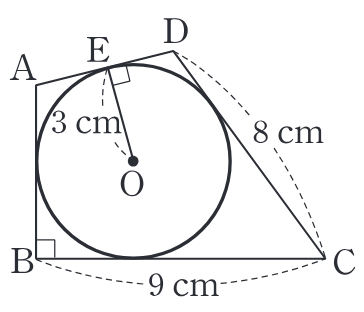
\includegraphics[width=\dmfigw]{figures/fig-0351.png}\end{minipage}\par
